\documentclass{article}
\usepackage{tikz}

\begin{document}

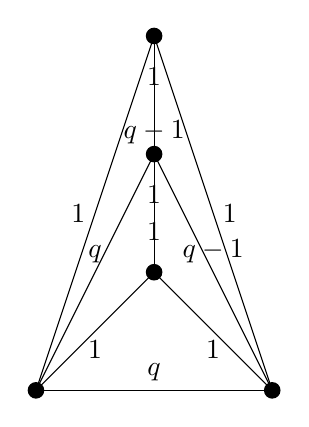
\begin{tikzpicture}[scale=1.5]
    % Define coordinates for the vertices
    \coordinate (A) at (0,0);
    \coordinate (B) at (2,0);
    \coordinate (C) at (1,3);
    \coordinate (D) at (1,1);
    \coordinate (E) at (1,2);

    % Draw the edges of the graph
    \draw (A) -- node[above] {$q$} (B);
    \draw (A) -- node[left] {$1$} (C);
    \draw (B) -- node[right] {$1$} (C);
    \draw (C) -- node[above] {$q-1$} (D);
    \draw (D) -- node[above] {$1$} (E);
    \draw (D) -- node[below] {$1$} (A);
    \draw (D) -- node[below] {$1$} (B);
    \draw (D) -- node[below] {$1$} (E);
    \draw (E) -- node[above] {$q-1$} (B);
    \draw (E) -- node[above] {$q$} (A);
    \draw (E) -- node[above] {$1$} (C);

    % Draw the vertices as filled circles
    \fill (A) circle (2pt);
    \fill (B) circle (2pt);
    \fill (C) circle (2pt);
    \fill (D) circle (2pt);
    \fill (E) circle (2pt);
\end{tikzpicture}

\end{document}